\subsection{Vision Transformer}\label{s:vit}
\chapterauthor{Low Hong Sheng Jovian (2203654)}

Vision Transformers (ViT) mark a crucial adaptation of transformer architectures from textual to image analysis \cite{Khan2021Transformers}. Initially designed for natural language processing, transformers employ self-attention mechanisms which are adeptly applied to visual data in ViTs. This adaptation enables the model to dynamically prioritize different image segments according to their relevance for tasks like tumor detection in brain MRI scans.

ViTs work by breaking down an image into fixed-size patches, embedding them linearly, and treating each as a token, similar to words in text processing \cite{Wu2020Visual} (see Figure \ref{fig:vit_architecture}). Positional embeddings are added to maintain spatial relationships. These embeddings are processed through multiple transformer layers, utilizing self-attention to analyze the image holistically, enhancing the detection of complex patterns and subtle nuances indicative of tumors.

\begin{figure}[H]
  \centering
  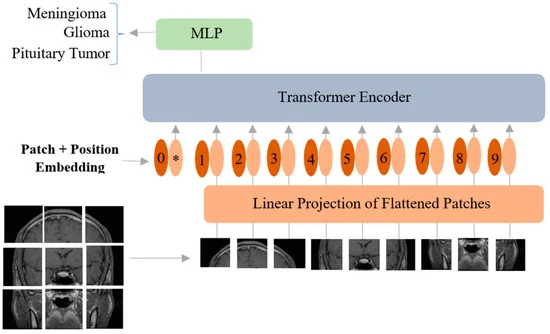
\includegraphics[width=0.45\textwidth]{vit/vit_architecture.png}
  \caption{ViT Architecture \cite{curroncol29100590}}
  \label{fig:vit_architecture}
\end{figure}

This method allows ViTs to excel in scenarios requiring deep contextual understanding and detailed image analysis. Particularly in medical imaging, ViTs are highly effective, often surpassing conventional CNNs by identifying less obvious features crucial for accurate diagnostics \cite{Matsoukas2021Is}.

Additionally, ViTs benefit from transfer learning, where models pre-trained on extensive general datasets are fine-tuned for specific medical tasks \cite{Simon2022Vision}. This not only reduces the need for large medical datasets but also speeds up the training process. Their adaptability and prowess in handling intricate image data make Vision Transformers a promising advancement in medical diagnostics, especially for improving the accuracy and reliability of brain tumor classifications.


\subsubsection{Implementation}

The proposed brain MRI classification model employs the Vision Transformer (ViT) architecture, pretrained on the ImageNet dataset. The Vision Transformer (ViT) represents a significant departure from traditional convolutional neural network models like InceptionV3, U-Net, and ResNet-50, primarily through its utilization of self-attention mechanisms. These mechanisms enable ViT to effectively capture and interpret the global context of an image, a capability that proves particularly valuable in the domain of medical image analysis, such as MRI scans. Unlike conventional models that rely on local receptive fields, ViT assesses all parts of the image in relation to one another, which can enhance the detection and classification of nuanced features within complex medical images. For application in MRI analysis, the ViT model is customized by removing its original classification head and adjusting its input size to $224\times224$ pixels with three channels, aligning it with the common dimensions of medical imaging datasets. This adaptation not only makes ViT a robust choice for this specific task but also necessitates careful training and parameter tuning to fully exploit its architectural benefits for medical diagnostics.

To specifically tailor the ViT model for brain MRI classification, the B16 variant is employed without its original classification head. The transformer's outputs undergo Global Average Pooling to condense the feature maps into a singular 768-dimensional vector, effectively capturing essential features while reducing dimensionality. To mitigate overfitting, a Dropout layer with a rate of 0.3 is incorporated. Further, a dense layer containing 512 neurons activated by ReLU leads to a final classification layer, which consists of four neurons. Each neuron corresponds to a different brain tumor class and utilizes a softmax activation function to provide the probabilities for each class, enhancing the model's ability to make accurate predictions on diverse MRI data.

The model leverages a custom Adam optimizer with a learning rate of 
$0.0001$. This choice is based on its empirical effectiveness in similar tasks involving high-dimensional image data, where stable and gradual adjustments to the weights are crucial. Additionally, the categorical cross-entropy loss function is utilized to address the multi-class nature of the classification challenge, ensuring that the model effectively discriminates between different brain tumor types.

To address class imbalance, a significant concern in medical datasets, the model training incorporates dynamically adjusted class weights. This strategy enhances the model's sensitivity to under-represented classes, thus improving its overall diagnostic accuracy. 
Training extends over 50 epochs with an early stopping mechanism that ceases training if there is no improvement in validation loss over 10 consecutive epochs. The optimal model is then preserved and further assessed on a validation set, where it achieved a peak training accuracy of 0.9974 and a validation accuracy of 0.9111, with the lowest validation loss recorded at 0.33246.


\subsubsection{Fine-Tuning}


% TO MOD THIS %
% In the process of fine-tuning the model, the Optuna package was utilized to conduct a comparative analysis of different optimizers, namely RAdam, Adam, and SGD. This hyperparameter optimization process aimed to identify the most effective optimizer for the final model. After extensive experimentation, RAdam was selected due to its superior performance in achieving higher validation accuracy compared to the other optimizers. This choice aligns with the findings of Khaliki et al. \cite{khaliki_brain_2024}, which highlight the advantages of RAdam in stabilizing training and enhancing convergence rates.

% In addition to optimizer selection, the dropout rate was also a subject of optimization attempts using the Optuna package. Despite exploring various dropout rates, the optimal dropout rate was found to be 0.055, which provided a balance between mitigating overfitting and maintaining model performance. This specific dropout rate was thus adopted in the final model architecture.

% The overall approach demonstrates the rigorous method employed to fine-tune the model, ensuring optimal performance for brain tumor segmentation. By leveraging advanced optimization techniques and thoroughly validating the model, this work contributes to the development of more accurate and reliable medical imaging models.

\subsubsection{Results and Evaluation}


The confusion matrices in Figures \ref{fig:inceptionv3_cm1} and \ref{fig:inceptionv3_cm2}, provide a detailed view of the model's performance across the four brain tumor classes: meningioma, pituitary, glioma, and no tumor. The pituitary and no tumor classes exhibit slightly lower but still commendable true positive rates of 0.88, indicating strong performance across all categories. The classification report in Table \ref{tab:inceptionv3_classification_report} summarizes the precision, recall, and F1-score for each class. The model demonstrates high precision and recall across all classes, with a notable F1-score of 0.96 for the meningioma class. The overall micro, macro, and weighted averages for precision, recall, and F1-score all stand at 0.93, reflecting consistent and reliable performance.

The ROC curve in Figure \ref{fig:inceptionv3_roc} displays the true positive rate against the false positive rate for each class. The areas under the curve (AUC) for pituitary and no tumor classes are both perfect at 1.00, while meningioma and glioma classes show AUCs of 0.97 and 0.99, respectively, indicating excellent discriminative ability of the model.

The learning curve in Figure \ref{fig:inceptionv3_learning_curve} illustrates the model's accuracy and loss over 100 epochs. The convergence of training and validation accuracy, alongside the decreasing trend in loss values, indicates effective learning without significant overfitting.

Table \ref{tab:inceptionv3_additional_metrics} highlights the Dice Similarity Coefficient (DSC), sensitivity, specificity, and accuracy of the model. The DSC of 0.9272 indicates a high overlap between the predicted and actual tumor regions. Sensitivity and accuracy, both at 0.9271, demonstrate the model's ability to correctly identify true positives, while the specificity of 0.9757 shows its effectiveness in correctly identifying true negatives.

\subsubsection{K-Folds Cross-Validation}

K-Folds cross-validation was performed to evaluate the model's performance across different subsets of the dataset. The model achieved an average validation accuracy of 0.9711 and an average validation loss of 0.2188 across five folds. The model was trained for 90 epochs with a batch size of 10 for each fold. The results demonstrate the model's consistency and robustness in classifying brain tumor images.

Results from K-Folds cross-validation are summarized in Figure \ref{f:inceptionv3_kfolds}, illustrating the validation accuracy and loss for each fold. The consistent performance across all folds, with minimal variance in accuracy and loss values, further validates the model's reliability and effectiveness in brain tumor segmentation tasks.

% Validation Accuracy: 0.9711 ± 0.0218
% Validation Loss: 0.2188 ± 0.0586
% k = 5
% epochs = 90 
% batch_size = 10


\subsubsection{Conclusion}


